\documentclass[compress,fleqn,utf8,aspectratio=169,t]{beamer}
% use LMU theme
\usetheme{LMU}

% This setups a lot of recommended settings and packages you usually need
% anyway. So let me take care for you and your document stays clear.

% Examples: Tables, Graphics, Listings, Hyperref...
%
% Prevent slide breaks in the middle of a paragraph
\widowpenalties 1 10000
\raggedbottom

\makeatletter
\@ifundefined{KOMAClassName}{% if non-KOMA class
  \IfFileExists{parskip.sty}{%
    \RequirePackage{parskip}
  }{% else
    \setlength{\parindent}{0pt}
    \setlength{\parskip}{6pt plus 2pt minus 1pt}}
}{% if KOMA class
  \KOMAoptions{parskip=half}}
\makeatother

\IfFileExists{xurl.sty}{\usepackage{xurl}}{} % add URL line breaks if available
\IfFileExists{bookmark.sty}{\usepackage{bookmark}}{\usepackage{hyperref}}
\urlstyle{same} % disable monospaced font for URLs

\usepackage{listings}
\lstset{defaultdialect=[5.3]Lua}
\lstset{defaultdialect=[x86masm]Assembler}
\usepackage{longtable,booktabs}
\usepackage{caption}
% Make caption package work with longtable
\makeatletter
\def\fnum@table{\tablename~\thetable}
\makeatother
\usepackage{graphicx}
\makeatletter
\def\maxwidth{\ifdim\Gin@nat@width>\linewidth\linewidth\else\Gin@nat@width\fi}
\def\maxheight{\ifdim\Gin@nat@height>\textheight\textheight\else\Gin@nat@height\fi}
\makeatother
% Scale images if necessary, so that they will not overflow the page
% margins by default, and it is still possible to overwrite the defaults
% using explicit options in \includegraphics[width, height, ...]{}
\setkeys{Gin}{width=\maxwidth,height=\maxheight,keepaspectratio}
% Set default figure placement to htbp
\makeatletter
\def\fps@figure{htbp}
\makeatother
\usepackage[normalem]{ulem}
% Avoid problems with \sout in headers with hyperref
\pdfstringdefDisableCommands{\renewcommand{\sout}{}}
\setlength{\emergencystretch}{3em} % prevent overfull lines
%Tightlist Command
\providecommand{\tightlist}{%
  \setlength{\itemsep}{0pt}\setlength{\parskip}{0pt}}


\usepackage[normalem]{ulem}
\usepackage{tikz}
\usetikzlibrary{shapes, arrows, automata, positioning, graphs, graphdrawing}
\usegdlibrary{trees, layered, force}
\usepackage[edges]{forest}
\usepackage{xcolor}
\usepackage{cancel}

\usepackage[style=ieee]{biblatex}
\addbibresource{main.bib}

\usepackage{lmodern}
\graphicspath{{./img/}}
% enable to get notes on the right (display with pympress)
% \setbeameroption{show notes on second screen=right}


%%%%%%%%%%%%%%%%%%%%%%%%%%%%%%%%%%%%%%%%%%%%%%%%%%%%%%%%%%%%%%%%%%%%%%%%%%%%%%%%
%%                                 Customizations                             %%
%%%%%%%%%%%%%%%%%%%%%%%%%%%%%%%%%%%%%%%%%%%%%%%%%%%%%%%%%%%%%%%%%%%%%%%%%%%%%%%%

% If you want navigation comment this
\beamertemplatenavigationsymbolsempty

% setup listings
\lstset{
  basicstyle=\ttfamily\color{black},
  showstringspaces=false
}

\lstdefinestyle{highlight}{
  keywordstyle=\color{red},
  commentstyle=\color{lmu@darkgray}
}

\lstdefinestyle{basetex}{
language={[LaTeX]Tex},
basicstyle=\color{black!40},
keywordstyle=\color{red!40},
commentstyle=\color{lmu@darkgray!40},
moredelim=**[il][\only<+>{\color{black}\lstset{style=highlight}}]{@}
}

\lstdefinestyle{basec}{
language=C,
basicstyle=\color{black!40},
keywordstyle=\color{red!40},
commentstyle=\color{green!40},
moredelim=**[il][\only<+>{\color{black}\lstset{style=highlight}}]{@}
}

%%%%%%%%%%%%%%%%%%%%%%%%%%%%%%%%%%%%%%%%%%%%%%%%%%%%%%%%%%%%%%%%%%%%%%%%%%%%%%%%
%%                                  Title Page Data                           %%
%%%%%%%%%%%%%%%%%%%%%%%%%%%%%%%%%%%%%%%%%%%%%%%%%%%%%%%%%%%%%%%%%
% helper command to add multiple authors
\newcommand{\newauthor}[2]{
\parbox[c]{0.26\textwidth}{
{\bfseries #1} \\
{\scriptsize{\href{mailto:#2}{#2}}}
}
% {#1}
}

% Authors
\author[Schmidt]{
  \newauthor{Adrian Schmidt}{adrian.schmidt@campus.lmu.de} \and
}

\institute[LMU]{
  % \inst{1}%
  {PD Dr. rer. nat. Vitalian Danciu\\}
  {Daniel Diefenthaler,}
  {Fabian Dreer,}
  {Cuong Tran}
  % \inst{2}%
  % {TUM}
}

% \date[\today]{\today}

% \title{MEADcast Evaluation utilizing a Linux Kernel Implementation of the Router}
% \title{MEADcast Evaluation:\\Linux Kernel Implementation of a Multicast Protocol}
% \title{MEADcast: Linux Kernel-Based Evaluation of a Multicast Protocol}
\title{MEADcast: Linux Kernel basierte Evaluation eines Multicast Protokolls}

% MEADcast: Evaluation of a Multicast Protocol implemented in the Linux Kernel
\subtitle{Masterarbeit Antrittspräsentation}
% \subtitle{Master's Thesis Entrance Presentation}

\hypersetup{
  pdftitle={Title},
  pdfauthor={Author},
  hidelinks}


%%%%%%%%%%%%%%%%%%%%%%%%%%%%%%%%%%%%%%%%%%%%%%%%%%%%%%%%%%%%%%%%%%%%%%%%%%%%%%%%
%%                                  Document                                  %%
%%%%%%%%%%%%%%%%%%%%%%%%%%%%%%%%%%%%%%%%%%%%%%%%%%%%%%%%%%%%%%%%%%%%%%%%%%%%%%%%

\begin{document}

\begin{frame}
	\titlepage
\end{frame}
% remove manual linebreak from title for correct footer rendering
% \title{MEADcast Evaluation: Linux Kernel Implementation of a Multicast Protocol}

\section{Einleitung}
\subsection{Kommunikationsformen} % (fold)
\label{sub:Multicast}
\begin{frame}{Kommunikationsformen}
\centering
    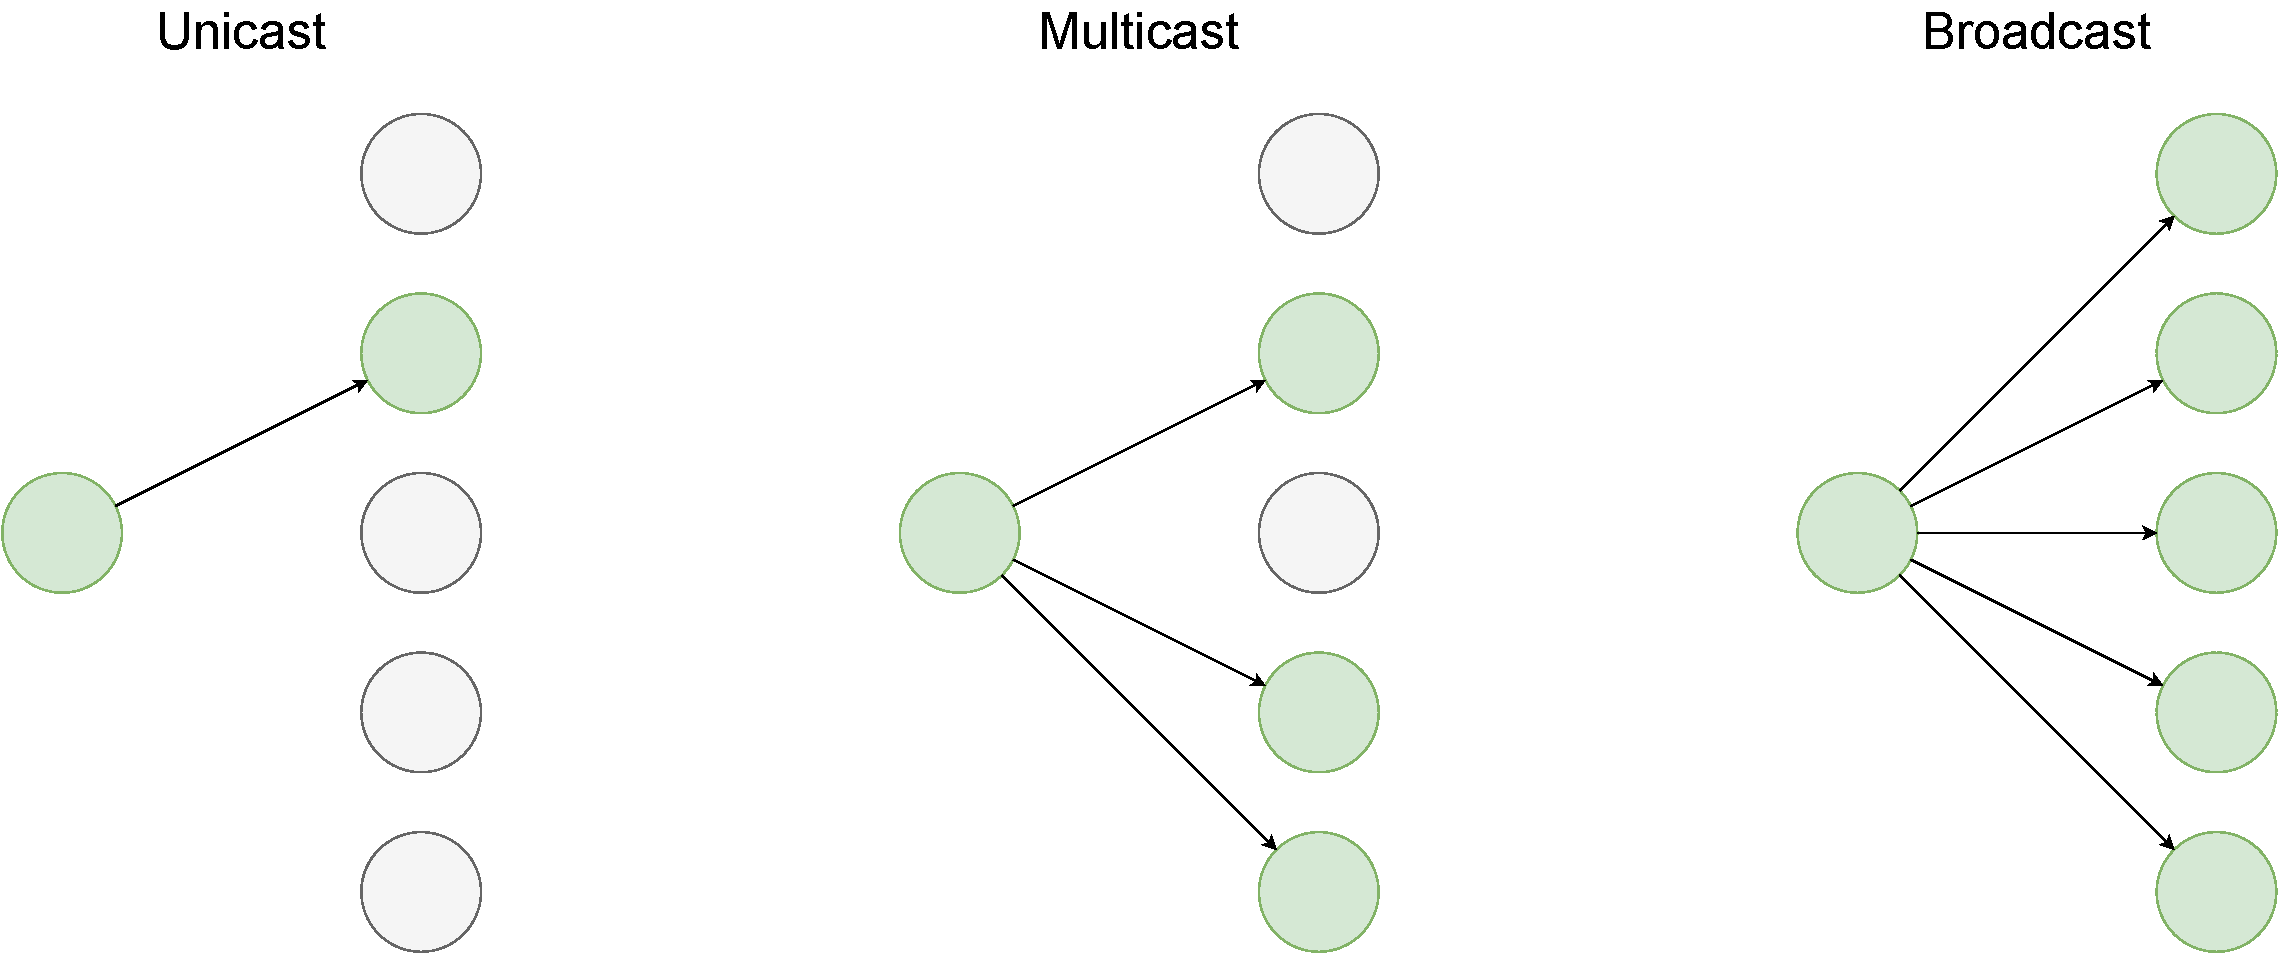
\includegraphics[width=.87\textwidth]{multicast.pdf}
\end{frame}
% subsection Multicast (end)

\subsection{Motivation}
\begin{frame}{Motivation}
	\begin{itemize}
        % \item Unrelenting growth of internet users and bandwidth consumption \cite{itu_digdev}
            % \note[item]{Over the past 5 years the average growth in total bw consumption was 30\%}
            % \note[item]{Further exelerated by COVID-19 pandemic}
		    % \note[item]{Especially servies such as Live Streams, Conferences,
                % and Online Gaming depict a major portion of the global traffic volume}
            % \note[item]{These services share the characteristics of:
            %     bandwidth intense, real-time, one-to-many or many-to-many
            %     $\Rightarrow$ make them well suited for multicast}
        % \item Many popular services are well-suited for multicast \cite{ratnasamy2006revisiting, meadcast1}
        % \item IP-Multicast serves efficient multipoint communication (\textit{1:m}, \textit{m:n}) \cite{deering1990multicast}
        % \item IP-Multicast is heavily used on a local scale \cite{rfc4861_ipv6_nd, rfc2453_rip}
		% \item Majority of internet traffic still relies on unicast (\textit{1:1})
        \item Internet Wachstum \& Bandbreitennutzung \cite{itu_digdev}
            \note[item]{Gesamte Bandbreitennutzung ist in den vergangenen 5 Jahren um durschnittlich 30\% gestiegen}
            \note[item]{Entwicklung durch COVID verstärkt}
            \note[item]{Besonders Dienste wie Live Streams, Video Konferenzen und Online Gaming
                bilden einen wesentlichen Bestandteil der globalen Internetverkehrs}
            \note[item]{Diese Dienste teilen sich ähnliche Charakteristiken:
                Bandbreiten intensive, Echtzeit, 1:n oder m:n
                $\Rightarrow$ gut geeignet für Mutlicast}
        \item Viele populäre Dienste sind gut geeignet für Multicast \cite{ratnasamy2006revisiting, meadcast1}
        \item IP-Multicast ermöglicht effiziente Multipunkt Kommunikation (\textit{1:n}, \textit{m:n}) \cite{deering1990multicast}
		% Well suited for the previously mentioned Characteristics
        \item Hohe Nutzung von Multicast in LANs \cite{rfc4861_ipv6_nd, rfc2453_rip}
            \note[item]{IPv6 Neighbor Discovery, Routing Protokolle wie RIP \& OSPF}
		\item Großteil des Internetverkehrs basiert auf unicast (\textit{1:1})
		% There are several reasons for that...
	\end{itemize}
\end{frame}

\subsection{Probleme von IP-Multicast} % (fold)
\label{sub:Challenges of IP-Multicast}
\begin{frame}{Probleme von IP-Multicast}
	\begin{itemize}
        % \item High technical complexity \cite{diot2000deployment}
            % \note[item]{requires the interaction of various protocols on multiple network layers}
        % \item Limited address space \cite{rfc1112_ip4mc, rfc4291_ip6mc}
            % \note[item]{Infeasible to map highly dynamic sessions onto address space}
        % \item Complex routing procedure \cite{diot2000deployment, ratnasamy2006revisiting}
            % \note[item]{Requires all routers along the path to maintain a per-session state}
		% \item Limited deployment by ISPs
            % \note[item]{ISPs not interested: more extensive mgm, infra upgrades, ...}
		% \item Limited urge for change
            % \note[item]{No impact on receivers $\Rightarrow$ not expected to exert pressure on ISPs.}
		% \item<2->[$\Rightarrow$] Various unicast-based alternatives have been
  %           developed, aimed at addressing the abesence of a globally usable
  %           multicast protocol.
        \item Hohe technische Komplexität \cite{diot2000deployment}
            \note[item]{Erfordert die Interaktion von diversen Protokollen auf unterschiedlichen Rechnernetz-Schichten}
        \item Limitierter Adressbereich \cite{rfc1112_ip4mc, rfc4291_ip6mc}
            \note[item]{Abbildung von dynamischen Sitzungen wie Video Konferenzen auf diesen Adressbreich nicht praktikabel}
        \item Komplexes Routingverfahren \cite{diot2000deployment, ratnasamy2006revisiting}
            \note[item]{Erfordert, dass alle Router entlang eines Pfades einen Sitzungsstatus pflegen}
		\item Limitierte Verfügbarkeit
            \note[item]{Netzbetreiber limitertes Interesse an Multicast: höherer administations Aufwand, Infrastruktur Upgrades, ...}
		% Not interested
		%   Higher Complexity --> More extensive mgm effort
		%   Infrastructure Upgrades
		%   Charging
		%   Anticipate Net load (Forecast number of replicas generated from a packet entering the network)
		\item Begrenzter Drang zur Veränderung
		% ISP not willing
            \note[item]{ISP limitiertes Interesse \& Mutlicast keinen direkt spürbaren Effekt auf Empfänger $\Rightarrow$ Es ist nicht zu erwarten, dass Kunden auf ISPs Druck ausüben}
		% Uniformed Client software (besides apps)
		\item<2->[$\Rightarrow$]
            Entwicklung diverser unicast-basierter alternativen, um (\textit{globale}) Gruppenkommuikation zu ermöglichen.
		  % Such as ALM, Xcast and MEADcast
	\end{itemize}
\end{frame}

% subsection Challenges of IP-Multicast (end)

\section{MEADcast} % (fold)
\label{sec:MEADcast}
\subsection{Überblick} % (fold)
\label{sub:Overview}
\begin{frame}{Überblick}
	\begin{itemize}
  %       \item 1:n sender-based IPv6 multipoint communication \cite{meadcast1, meadcast2}
		% \item Based on IPv6-unicast, encodes destinations in IP Extension Header
		% \item MEADcast router replicate packets
		% \item Key features:
  %           \note[item]{The protocol focuses on Privacy \& Availability}
		%       \begin{itemize}
		% 	      \item preservation of receiver privacy
  %                     \note[item]{Xcast \& ALM disclose Endpoint IPs}
		% 	      \item technology-agnostic destinations
		% 	            % Closest MEADcast router transforms MEADcast packet to usual IPv6 unicast packet
		% 	      \item zero network support requirements
  %                     \note[item]{Fallback mechanism to unicast}
		%       \end{itemize}
        \note[item]{Hier am Lehrstuhl entwickelt!}
        \item 1:n Sender-basiertes Multicast Protokoll \cite{meadcast1, meadcast2}
        \item Basierend auf IPv6-unicast; kodiert Zieladressen in IPv6 Extension Header
		\item MEADcast Router replizieren Pakete
		\item Zentrale Eigenschaften:
            \note[item]{Das Protokoll fokussiert sich auf Privacy \& Verfügbarkeit}
		      \begin{itemize}
			      \item Schutz der Empfänger Privatsphäre 
                      \note[item]{Verwandte Protokolle teilen Endpunkt Infos wie IPs unter den Empfänger}
			      \item Keine Empfänger Unterstützung notwendig
			            % Closest MEADcast router transforms MEADcast packet to usual IPv6 unicast packet
			      \item Keine Rechnernetz Unterstützung notwendig
                      \note[item]{MEADcast ist unicast $\Rightarrow$ wird ohnehin gerouted}
                      \note[item]{Fallback Mechanismus zu normalem unicast}
		      \end{itemize}
	\end{itemize}
\end{frame}
% subsection MEADcast (end)

% section MEADcast (end)


\section{Ziel \& Beitrag} % (fold)
\label{sec:Goal and contribution}
\subsection{Ziel}
\begin{frame}{Ziel}
	% MEADcast evaluation utilizing a Linux Kernel implementation of the router
	% software.
 %    \note[item]{Represents logical progression from earlier investigations of MEADcast,
 %        which were based on network simulations and SDNs}
 %    \note[item]{The evaluation primarily focuses on:}
	% \begin{itemize}
	% 	\item<2-> Feasibility
 %            \note<2->[item]{Gap between realilty and simulation}
 %            \note<2->[item]{Working in simulations doesn't imply it works in a real network nor on the internet}
 %            \note<2->[item]{Structural issues? Deployment issues? Does it work on the internet? Intermediate Firewalls?}
	% 	\item<3-> Performance (compared to IP uni- \& multicast)
 %            \note<3->[item]{MEADcast comes with some addtional overhead compared to IP-Multicast:}
 %            \note<3->[item]{What is the impact of this overhead?}
 %            \note<3->[item]{Total transfered bytes, Throughput, Latency, Jitter, Router load}
	% 	\item<4-> Scenario Identification
 %            \note<4->[item]{Under which conditions its sensible to use MEADcast?}
 %            \note<4->[item]{Which application characteristics? (e.g. small vs. big groups, short vs. long sessions, endpoint distro, ...)}
	% 		% Under which conditions it performs good?
	% \end{itemize}
	MEADcast Evaluation basierend auf einer Linux Kernel Implementierung des Routers.
    \note[item]{Knüpft an vorherige Untersuchungen von MEADcast an, welche auf Simulationen und SDNs basierten}
    \note[item]{Primärer Fokus auf 3 Punkte:}
	\begin{itemize}
		\item<2-> Nutzbarkeit / Umsetzbarkeit
            \note<2->[item]{Unterschiede zwischen Simulation und Realität}
            \note<2->[item]{Nutzbarkeit in Simulation impliziert nicht Nutzbarkeit in echten Rechnernetzen}
            \note<2->[item]{Strukturelle Probleme der aktuellen Protokoll Spezifikation? Deployment? Verfügbarkeit im Internet? Firewalls?}
		\item<3-> Performance (versus IP uni- \& multicast)
            \note<3->[item]{MEADcast bringt Overhead im Vgl. zu Multicast mit sich:}
            \note<3->[item]{Wie groß ist der Einfluss des Overheads?}
            \note<3->[item]{Übertragene Bytes, Durchsatz, Latenz, Jitter, Router/Sender Last}
		\item<4-> Szenario Identifikation
            \note<4->[item]{Unter welchen Umständen ist der Einsatz von MEADcast sinnvoll?}
            \note<4->[item]{Welche Anwendung eignen sich? Welche Charakteristiken? (e.g. kleine vs. große Gruppen, kurze vs. lange Sitzungen, Verteilung der Endpunkte, ...)}
			% Under which conditions it performs good?
	\end{itemize}
\end{frame}


\subsection{Beitrag} % (fold)
\label{sub:Contribution}
\begin{frame}{Beitrag}
	\begin{itemize}
		% \item Linux Kernel implementation of the MEADcast router.
		% \item Implementation of a traffic generator acting as the sender.
		% \item Deployment of MEADcast in both a testbed and a real network
		% \item Evaluation of MEADcast's feasibility, performance, and potential
		%       application scenarios.
  %       \item Potential proposal for a revision of the MEADcast specification.
		\item Linux Kernel Implementierung der Router Software
            \note[item]{Ermöglicht den Einsatz für Anwendungen in realen Rechnernetzen}
        \item Prototypische Sender Implementierung
            \note[item]{Sender simuliert die Verwendung von MEADcast}
		\item Deployment von MEADcast in kontrollierten Testbed sowie realen Rechnernetz
        \item MEADcast Evaluation hinsichtlich Nutzbarkeit, Performance \& potentieller
		      Anwendungsfälle
            \note[item]{Wertvolle Einblicke in zukünftigen Einsatz \& Entwicklung}
        \item Vorschlag für nächste Revision der Protokoll Spezifikation
	\end{itemize}
\end{frame}

% section Goal \& Contribution (end)
% % subsection Contribution (end)

\section{MEADcast}
\subsection{IP Extension Header} % (fold)
\label{sub:IP Extension Header}
\begin{frame}[c]{IP Extension Header}
\centering
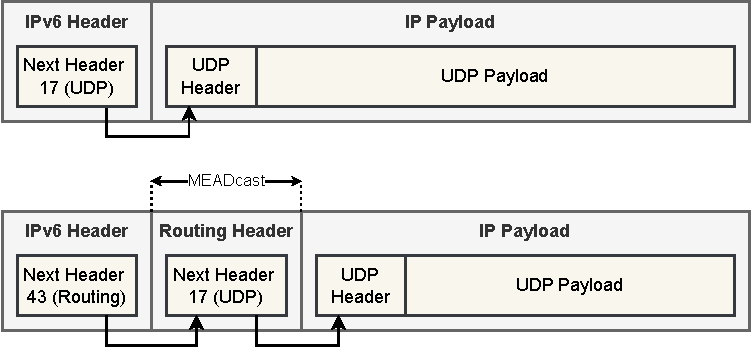
\includegraphics[width=.6\textwidth]{exthdr.pdf}
\end{frame}
% subsection IP Extension Header (end)


\begin{frame}[c]{Datenübertragung}
    \note[item]{1 Sender Daten an 3 EPs via MEADcast übertragen}
    \note[item]{Discovery- \& Datenübertragungsphase}
    \note[item]{Discovery: MEADcast Paket an jeden EP $\rightarrow$ Router antworten, parallel Unicast übertragung}
    \note[item]{Sender kennt alle Router \& wechselt auf MEADcast Übertragung}
    \centering
	%  \tikz \graph [tree layout, nodes={inner sep=1pt,draw,circle},
	%            component direction=up]
	% { a, b, c [grow=right] -- d -- e, f[grow=45] -- g };

	% \tikz \graph [tree layout, grow=right]
	% {
	%     S->R1->{
	%         R2->{E2},
	%         E1
	%     }
	% };

	% \begin{tikzpicture}
	%     [->,>=stealth',shorten >=1pt,node distance=3cm,auto,font=\footnotesize]
	% \node[state] (S) {$S$};
	% % \node[state, right=+2cm of S] (R1) {$R_1$};
	% \node[state, right of =S] (R1) {$R_1$};
	% \node[state, above right of =R1] (E1) {$E_1$};
	% \node[state, below right of =R1] (R2) {$R_2$};
	% \node[state, right of =R2] (E2) {$E_2$};
	% \node[state, right of =R2] (E2) {$E_2$};
	%
	%     \path[font=\scriptsize]
	%         (S)  edge              node[align=center] {(S,R1,E1,R2,E2)} (R1)
	%         (R1) edge              node {unicast} (E1)
	%         (R1) edge              node {(S,\sout{R1},\sout{E1},R2,E2)} (R2)
	%         (R2) edge              node {unicast} (E2)
	%         ;
	% \end{tikzpicture}

    \begin{forest}
        for tree={grow=east, circle, draw, fill=black!8, font=\scriptsize},
            where level=0{ l sep+=55pt}{},
            where level=1{
                l sep+=55pt,
                s sep+=10pt}{},
            where level=2{
                l sep+=25pt,
                s sep+=10pt}{}
            [$S_1$
                [$R_1$,
                thick,
                edge label={node[midway,above,sloped,font=\tiny]{
                    ($\underline{R_2}$,$E_1$,$\underline{R_3}$,$E_2$,$E_3$)
                }}
                    [$R_3$,
                thick,
                edge label={node[midway,below,sloped,font=\tiny]{
                    ($\underline{\cancel{R_2}}$,$\cancel{E_1}$,$\underline{R_3}$,$E_2$,$E_3$)
                }}
                        [$E_3$,
                edge label={node[midway,below,align=center,font=\tiny]{
                    unicast
                }}
                        ]
                        [$E_2$,
                edge label={node[midway,above,align=center,font=\tiny]{
                    unicast
                }}
                        ]
                    ]
                    [$R_2$,
                thick,
                edge label={node[midway,above,sloped,font=\tiny]{
                    ($\underline{R_2}$,$E_1$,$\underline{\cancel{R_3}}$,$\cancel{E_2}$,$\cancel{E_3}$)
                }}
                        [$E_1$,
                edge label={node[midway,above,align=center,font=\tiny]{
                    unicast
                }}
                        ]
                    ]
                ]
            ]
    \end{forest}
\end{frame}


% \section{Method} % (fold)
% \label{sub:Method}
% \begin{frame}[t]
% \begin{columns}[T]
% \column{.3\textwidth}
% \only<1>{ 
%     Problem analysis:
%     \begin{itemize}
%         \item Technical challenges
%         \item Desireablility
%     \end{itemize}
% }
% \only<2>{
%     Goal:
%     \begin{itemize}
%         \item Feasibility
%         \item Performance
%         \item Application scenarios
%     \end{itemize}
% }
% \only<3>{
%     Metrics:
%     \begin{itemize}
%         \item Feasibility: 
%         \item Performance
%         \item Application scenarios
%     \end{itemize}
% }
% \column{.7\textwidth}
% % \centering
% \begin{tikzpicture}
% [auto,font=\footnotesize,
% % STYLES
% every node/.style={node distance=.8cm},
% comment/.style={rectangle, inner sep= 2pt, text width=4cm, node distance=0.25cm, font=\tiny\sffamily},
% force/.style={rectangle, rounded corners, draw, fill=black!8, text width=2cm, text badly centered, minimum height=.7cm, font=\bfseries\tiny\sffamily}]
%
% \node[force]                                                           (problem)       {Problem analysis};
% \node<2->[force, below of=problem,         right=-1.2cm of problem]       (goal)          {Goal definition};
% \node<3->[force, below of=goal,            right=-1.2cm of goal]          (criteria)      {Metric \& Criteria selection};
% \node<4->[force, below of=criteria,        right=-1.2cm of criteria]      (design)        {Experiment design};
% \node<5->[force, below of=design,          right=-1.2cm of design]        (requirements)  {Requirements analysis};
% \node<6->[force, below of=requirements,    right=-1.2cm of requirements]  (testbed)       {Testbed design};
% \node<7->[force, below of=testbed,         right=-1.2cm of testbed]       (experiment)    {Experiment conduction};
% \node<8->[force, below of=experiment,      right=-1.2cm of experiment]    (evaluation)    {Evaluation};
%
% \draw<2->[-latex,thick] (problem.south west)        +(7mm,0) |- (goal.west);
% \draw<3->[-latex,thick] (goal.south west)           +(7mm,0) |- (criteria.west);
% \draw<4->[-latex,thick] (criteria.south west)       +(7mm,0) |- (design.west);
% \draw<5->[-latex,thick] (design.south west)         +(7mm,0) |- (requirements.west);
% \draw<6->[-latex,thick] (requirements.south west)   +(7mm,0) |- (testbed.west);
% \draw<7->[-latex,thick] (testbed.south west)        +(7mm,0) |- (experiment.west);
% \draw<8->[-latex,thick] (experiment.south west)     +(7mm,0) |- (evaluation.west);
%
% % \node<2-2>[comment, right=0.2 of problem]{
% %     $\bullet$\quad Technical challenges\\
% %     $\bullet$\quad Desireablility
% % };
% % \node<4->[comment, right=0.2 of goal]{
% %     $\bullet$\quad Feasibility\\
% %     $\bullet$\quad Performance\\
% %     $\bullet$\quad Scenarios\\
% % };
%
% \end{tikzpicture}
% \end{columns}
% \end{frame}
% % section Method (end)


% section Method (end)
\section{Methode} % (fold)
\label{sub:Method}
\begin{frame}%[c]
	% \centering
	\begin{columns}[T]
		\column{.17\textwidth}
		\column{.93\textwidth}
		\begin{tikzpicture}
			[auto,font=\footnotesize,
				% STYLES
				every node/.style={node distance=.8cm},
				force/.style={rectangle, rounded corners, draw, fill=black!8, text width=2cm, text badly centered, minimum height=.7cm, font=\bfseries\tiny\sffamily}]

			\node[force]                                                          (problem)       {Problemanalyse};
			\node<2->[force, below of=problem,         right=-1.2cm of problem]       (goal)          {Zielformulierung};
			\node<3->[force, below of=goal,            right=-1.2cm of goal]          (criteria)      {Metrik \& Kriterien Auswahl};
			\node<4->[force, below of=criteria,        right=-1.2cm of criteria]      (design)        {Experiment Design};
			\node<5->[force, below of=design,          right=-1.2cm of design]        (requirements)  {Anforderungsanalyse};
			\node<6->[force, below of=requirements,    right=-1.2cm of requirements]  (testbed)       {Testbed Design};
			\node<7->[force, below of=testbed,         right=-1.2cm of testbed]       (experiment)    {Datenerhebung};
			\node<8->[force, below of=experiment,      right=-1.2cm of experiment]    (evaluation)    {Evaluation};

			\draw<2->[-latex,thick] (problem.south west)        +(7mm,0) |- (goal.west);
			\draw<3->[-latex,thick] (goal.south west)           +(7mm,0) |- (criteria.west);
			\draw<4->[-latex,thick] (criteria.south west)       +(7mm,0) |- (design.west);
			\draw<5->[-latex,thick] (design.south west)         +(7mm,0) |- (requirements.west);
			\draw<6->[-latex,thick] (requirements.south west)   +(7mm,0) |- (testbed.west);
			\draw<7->[-latex,thick] (testbed.south west)        +(7mm,0) |- (experiment.west);
			\draw<8->[-latex,thick] (experiment.south west)     +(7mm,0) |- (evaluation.west);
            \draw<9->[-latex,dotted] (experiment.north east)  +(-3mm,0) to[bend right] (testbed.east);
            \draw<9->[-latex,dotted] (experiment.north east)  +(-3mm,0) to[bend right] (requirements.east);
            \draw<9->[-latex,dotted] (experiment.north east)  +(-3mm,0) to[bend right] (design);
		\end{tikzpicture}
	\end{columns}

% NOTES:
% \note[item]{Current State \& challenges of global multipoint communication}
% \note<2->[item]{MEADcast's Feasibility, performance, and potential application scenarios}
% \note<3->[item]{Performace: Total number of transfered packets/bytes, throughput, Latency, jitter}
% \note<4->[item]{Send MEADcast over the internet}
% \note<4->[item]{Simulate typical video conference}
% % 5) Derive testbed requirements from experiments
% % 6) Design testbed according to requirements
% %       - Network Topology
% %       - Intermediate Firewall
% % 7) Conduct Experiments
% \note<7->[item]{Probably XEN or KVM based}
% % 8) Evaluate with respect to the goal.
% \note<8->[item]{Provides valuable insights into feasibility and performance of MEADcast}
% \note<8->[item]{This analysis allows us to identify scenarios and applications for
%           which the protocol is well-suited}
\note[item]{Ausgangssituation \& Probleme/Herausforderung von (globaler) Multicast Kommunikation}
\note<2->[item]{MEADcasts Nutzbarkeit, Performance \& potentielle Anwendungsfälle}
\note<3->[item]{Performace: Übertragene Bytes/Packete, Durchsatz, Latenz, jitter, ...}
\note<4->[item]{MEADcast Pakete über das Internet versenden}
\note<4->[item]{Simulation einer klassischen Videokonferenz}
% 5) Derive testbed requirements from experiments
% 6) Design testbed according to requirements
%       - Network Topology
%       - Intermediate Firewall
% 7) Conduct Experiments
\note<6->[item]{Wahrschl. KVM oder XEN}
% 8) Evaluate with respect to the goal.
\note<8->[item]{Wertvolle Infos über Verfügbarkeit und Performance von MEADcast}
\note<8->[item]{Analyse ermöglicht uns die Identifikation von Szenarien und
    Apps., für welche MEADcast gut geeignet ist}

\end{frame}
% section Method (end)

\section{Zeitplan} % (fold)
\label{sec:Time Schedule}
\begin{frame}[c]
\centering
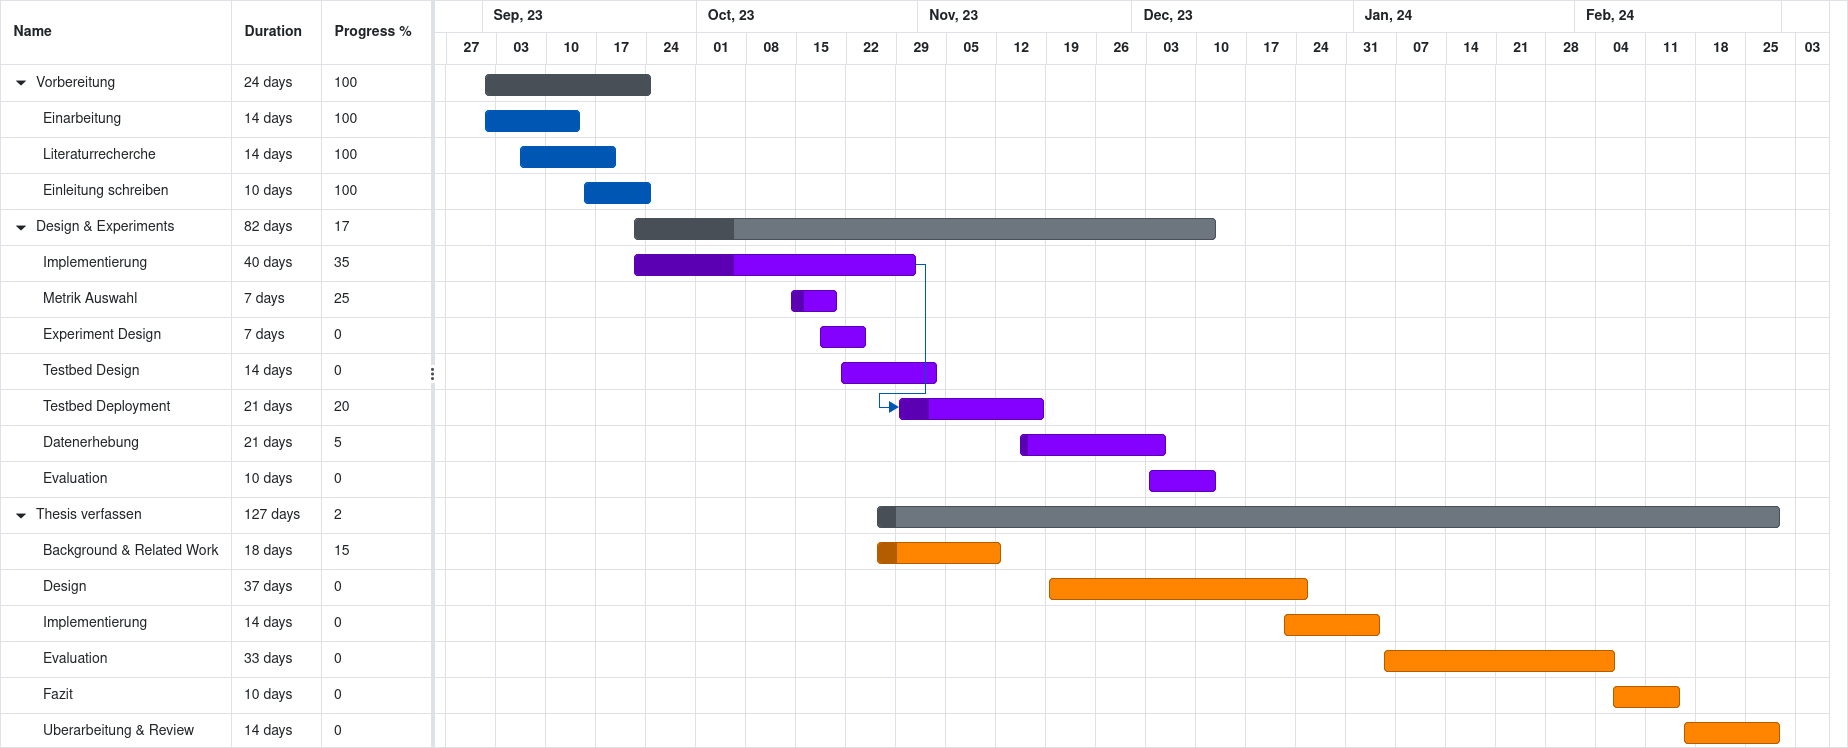
\includegraphics{schedule.png}
\end{frame}
% section Time Schedule (end)
\end{document}
